% E10 supplementary fragment; existing manuscript is not modified.
\subsection{E10: Parameter-matched local spatial interaction control}
\paragraph{Methods.}
We added SPATIAL\_MIXER\_MATCHED to distinguish local spatial interaction
from the graph-based reasoning used by FULL. The control retains the
NO\_GRAPH frontend, evidence fusion, $768\to256$ token projection and
joint heads. Projected tokens are reshaped to a $14\times14$ grid and
processed by two residual blocks, each comprising channel-only LayerNorm,
a $3\times3$ depthwise convolution (padding 1), a $1\times1$ expansion
from 256 to 832 channels, GELU and a $1\times1$ projection to 256 channels.
The width was selected by parameter count alone before training.
The control has 1,416,100 trainable parameters, versus 1,416,490 for FULL
(a 0.0275\% difference); decoder and pretrained ViT weights are frozen.
The existing E2 Train/Validation split, payloads, attacks, loss and
optimization rules are reused. Seeds 20261001--20261003 are paired with
the completed E2 runs. Each new control is initialized independently;
no trainable FULL weights are used. Checkpoints minimize Validation
joint loss; detection thresholds maximize Validation Youden J, and
the localization threshold is 0.5. Validation therefore participates
in selection and is not a new blind test. Test, CASIA2 and E9 are not evaluated.

\paragraph{Results.}
FULL achieved micro pixel $F_1$ $0.7574\pm0.0070$, while the spatial mixer achieved $0.7082\pm0.0075$. Values are means $\pm$ sample standard deviations across three seeds. The three paired FULL-minus-spatial-mixer pixel-$F_1$ differences were +0.0462, +0.0494 and +0.0519; their mean was +0.0492 with sample standard deviation 0.0029. All three paired localization differences favored FULL on this fixed Validation split. This supports a FULL advantage over this particular local convolution control, but does not establish a general or topology-specific advantage.

\paragraph{Limitations.}
This control matches trainable parameter count, not FLOPs or runtime.
Two local convolution blocks have a finite receptive field, whereas
FULL includes spatial and appearance-based graph communication.
Only three training seeds and one previously used Validation split
are available; the sample standard deviations are not independent-test
confidence intervals. No population-level significance or exclusive
causal role of graph topology is claimed.

\begin{table*}[!tbp]
\centering
\caption{E10 and existing E2 controls on IMD2020 Validation. Mean $\pm$
sample SD across three paired training seeds. Pixel metrics pool counts
within each run; Validation selects checkpoints and detection thresholds.}
\label{tab:e10_spatial_mixer}
\small
\begin{tabular}{@{}lrrrrr@{}}
\toprule
Model & Trainable parameters & AUC & Detection $F_1$ & Pixel $F_1$ & IoU \\
\midrule
FULL & 1,416,490 & $0.9948\pm0.0044$ & $0.9808\pm0.0048$ & $0.7574\pm0.0070$ & $0.6095\pm0.0092$ \\
NO\_GRAPH & 555,812 & $0.9856\pm0.0026$ & $0.9700\pm0.0048$ & $0.7217\pm0.0072$ & $0.5646\pm0.0088$ \\
Matched NO\_GRAPH & 1,416,110 & $0.9869\pm0.0021$ & $0.9838\pm0.0002$ & $0.6951\pm0.0376$ & $0.5336\pm0.0439$ \\
SPATIAL\_MIXER\_MATCHED & 1,416,100 & $0.9863\pm0.0005$ & $0.9752\pm0.0000$ & $0.7082\pm0.0075$ & $0.5483\pm0.0091$ \\
\bottomrule
\end{tabular}
\end{table*}

\begin{figure*}[!tbp]
\centering
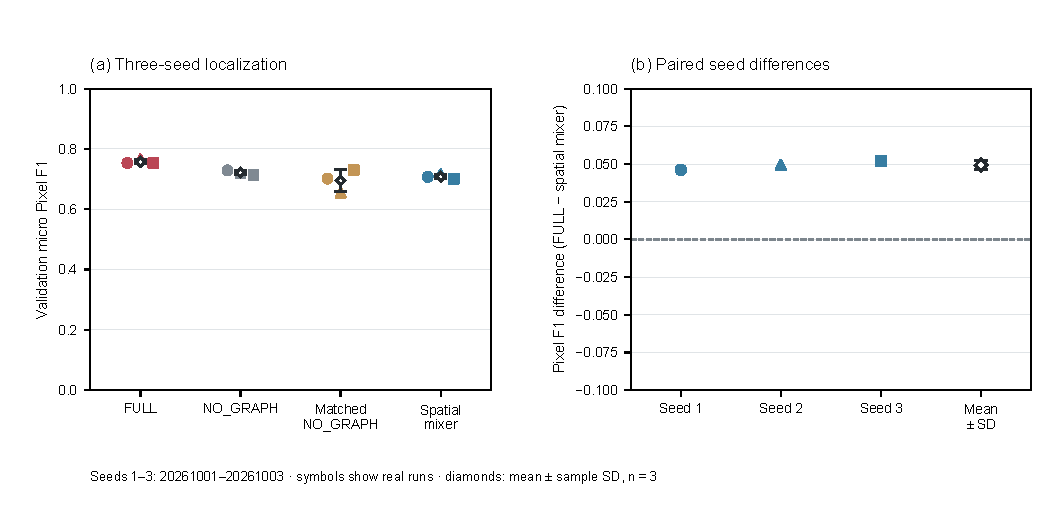
\includegraphics[width=\textwidth]{figure_e10_comparison.pdf}
\caption{E10 local spatial interaction control. (a) Three actual training
seed results per model, with diamonds and error bars denoting mean
$\pm$ sample SD. (b) Three paired FULL-minus-spatial-mixer pixel-$F_1$
differences and their mean $\pm$ sample SD. Marker shapes identify
seeds 20261001--20261003. All results use the same 124-sample
IMD2020 Validation cohort; no sample or seed is excluded.}
\end{figure*}

\begin{figure*}[!tbp]
\centering
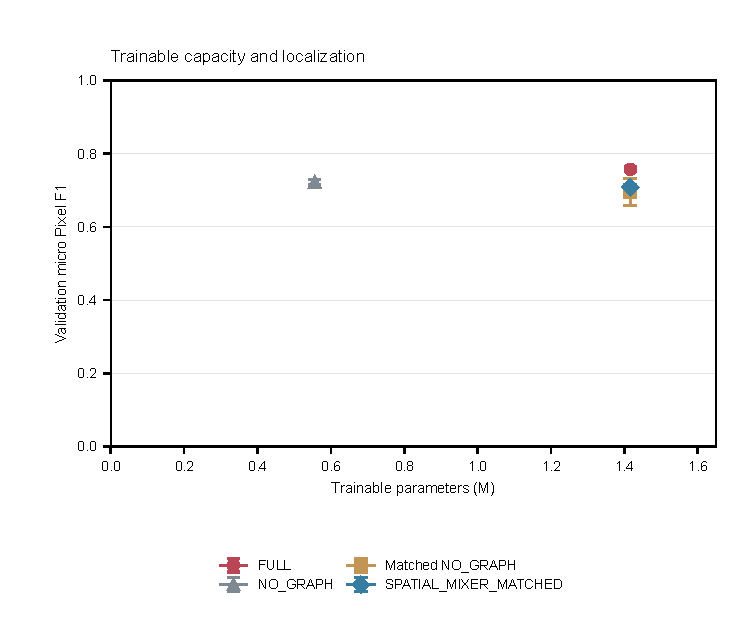
\includegraphics[width=0.70\textwidth]{figure_e10_parameters.pdf}
\caption{Trainable parameter count versus micro pixel $F_1$.
Each point is a three-seed mean, with sample SD error bars.
FULL, Matched NO\_GRAPH and SPATIAL\_MIXER\_MATCHED have nearly
identical x-coordinates because their trainable parameter counts
are closely matched. Frozen decoder and ViT parameters are excluded.}
\end{figure*}
